\documentclass[letterpaper, 12pt]{book}
\hfuzz=9.002pt
\usepackage{listings}
\usepackage{graphicx}
\usepackage{qrcode}
\usepackage{color}
\usepackage{xcolor}
\usepackage{amsmath}
\usepackage{hyperref}
\hypersetup{
    linktoc=all
}
\definecolor{theWhite}{gray}{0.9}
\lstset{
	breaklines=true,
	language=C++,
	backgroundcolor=\color{theWhite},
	basicstyle=\color{white},
	numbers=left,
	stepnumber=1,
	showstringspaces=false,
    basicstyle=\ttfamily,
    keywordstyle=\color{blue}\ttfamily,
    stringstyle=\color{red}\ttfamily,
    commentstyle=\color{green}\ttfamily,
    morecomment=[l][\color{magenta}]{\#},
    tabsize=4,
    literate={\ \ }{{\ }}1
}
\usepackage{epigraph}
\setlength \epigraphwidth {\linewidth}
\setlength \epigraphrule {0pt}
\AtBeginDocument{\renewcommand {\epigraphflush}{center}}
\renewcommand {\sourceflush} {center}
\hyphenpenalty=10000
\newtheorem{remark}{Remark}
\newtheorem{definition}{Definition}
\begin{document}
\date{}
\title{Byte Club's Computer Science with C++}
\author{Aryan Mediratta}
\maketitle
\tableofcontents
\chapter*{Introduction}
Hello friend. Welcome to your amazing journey to this new world of Computer Science. This is my attempt to simplify Computer Science to a level at which the information is both decently accurate and easy to understand. I hope you will enjoy learning and find some application of this knowledge in the real life. Computer Science is no less than an adventure to a land you've not been to before, and therefore, I want you to feel the excitement as we begin to take a look at what awaits us.\\
Another thing I would like to mention is that my goal here is not being highly accurate. Instead, my goal here, is to be easy to understand. When you teach someone math for the first time, you don't begin with Calculus. You start with counting and arithmetic with simple whole numbers. When someone new to mathematics tries to subtract a bigger number from a smaller one, we initially tell them it's not possible (i.e. it makes no sense) and later explain that negative numbers exist.\\
This is my goal here - Removing all the clutter and going through the foundational building blocks of computer science.\\
Also, I've attempted to write this book in first person, since I have often noticed that when authors write books in third person, the readers tend to feel a sense of disconnection from both the author and the subject. And that is where I feel most textbooks have gone wrong. This is thus my experiment to try filling this gap between learners and the book.\\
With that said, I wish you luck for your visit to this new world.\\
\begin{flushright}
\textbf{May the code be with you!}
\end{flushright}
\chapter{An Introduction to C++}
\epigraph{\centering ``C makes it easy to shoot yourself in the foot; C++ makes it harder, but when you do it blows your whole leg off."}{\textit{Bjarne Stroustrup \\ The Creator of C++}}
\section{Why C++?}
This is the very first chapter of the book and I'm talking directly about C++. Is that weird? Many people would have told you that C++ is difficult and that Python is the language to start with. I totally disagree with that opinion. You see, the thing is that Python is so overly simple that if we use it to learn computer science, it won't teach us a lot. You'll realize it later that Python has what I like to call ``Magic". And while there's no harm in seeing magic happen, the real fun is in doing that magic yourself. C++ doesn't have much ``magic" built-in. This allows us to \textbf{do the ``magic" ourselves} And trust me, it's going to be awesome.
\section{Some HiSTORY}
History is boring, isn't it? Well, yes, if you get stuck with the dates and the facts. However, in this case, I'll remove all the boring parts of it. All we care about, is the story of C++. Let's begin.
\subsection{Assembly}
You must have learnt in your previous classes that the computer understands only one language. No prizes for guessing - \textbf{Binary}. It's either a zero or a one, i.e. on or off.\\
However, that's not the complete story. A computer understands binary, but that binary code is actually just a way of writing a language called \textbf{Assembly}, also known as \textbf{Machine Code}.\\ 
But Assembly is not an easy thing to learn. In order to solve this problem, the B Programming language was created.
\subsection{The B Programming Language}
To tackle this problem, Ken Thompson and Dennis Ritchie at Bell Labs created a programming language called \textbf{B}. It worked at a higher level of abstraction than Assembly and helped people program using expressions with English words. All code written in this language had to ultimately be compiled (converted) to Assembly in order to be executed. They named it B, considering it a sequel to the BCPL (Basic Combined Programming Language), which was also a very low level language similar to Assembly.
\subsection{The C Programming Language}
Later, Dennis Ritchie created another new programming language called \textbf{C}. B was a typeless programming language. C solved this problem by introducing a type system. It remained and is still considered very influential in the world of programming. After some years, a new way (paradigm) of programming emerged. It was called the Object Oriented Programming System (OOPS). C, being an old language, did not support it, although it could do the low level work much better than the new languages.
\subsection{The C++ Programming Language}
Soon, Bjarne Stroustrup at Bell Labs solved this problem by making yet another language called \textbf{C++}. It was basically ``C with classes". We'll learn about classes later. They are basically the foundational concept behind OOPS. Note that most things valid in C are also valid in C++. The name C++ itself is a nice joke which you'll learn about later in this book.
\pagebreak
\subsection{The people we talked about}
\begin{figure}[h]
\centering
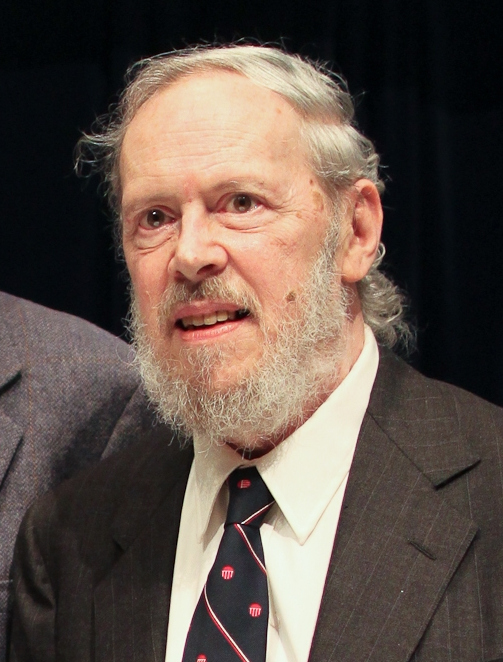
\includegraphics[width=3cm]{img/ritchie}
\caption{Dennis Ritchie}\label{ritchie}
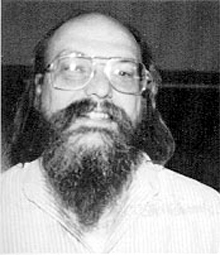
\includegraphics[width=3cm]{img/kenthompson}
\caption{Ken Thompson}\label{kenthompson}
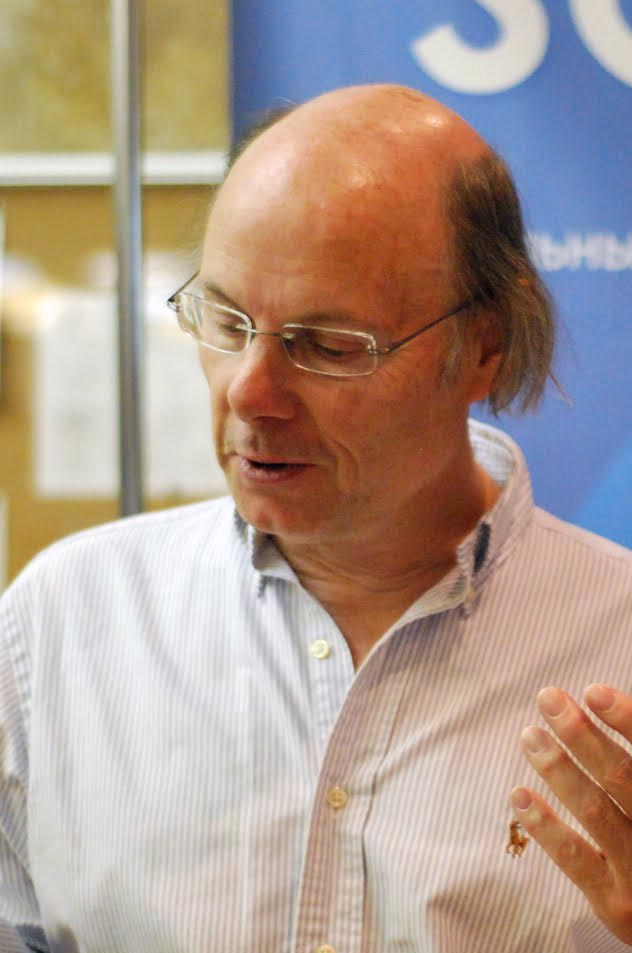
\includegraphics[width=3cm]{img/stroustrup}
\caption{Bjarne Stroustrup}\label{stroustrup}
\end{figure}
\section{Setting Things Up}
We shall now set up our C++ development environment. We will write C++ in an IDE (Integrated Development Environment) called Visual Studio 2019. It is a very powerful IDE from Microsoft and will help us in easy debugging.\\
At the time of writing this, Visual Studio 2019 is in the Preview (Testing) phase. However, our interface should look more or less the same. If you are reading this when a newer version of Visual Studio (i.e. above 2019) is available, please prefer the latest version.\\
If you do not like Microsoft or Visual Studio for some reason, you can feel free to use whatever C++ compiler and distribution you like (Suggestion: if not Visual Studio, try CLion - it's free for students). Just make sure you have a debugger.\\
Also, I must say this in uppercase: STAY AWAY FROM TURBO C++!
\subsection{Installing Visual Studio}
From a browser, head over to https://visualstudio.microsoft.com/vs/ and download the setup for Visual Studio 2019 Community.\\ Run the setup and when it asks you for selecting the components, choose ``Desktop Development with C++".\\
Allow it to download and install Visual Studio. It may take quite long, based on your internet connection. However, believe me, it's totally worth the wait :).\\
If you still need help with the setup, you can scan this QR code and/or visit this YouTube link:\\
\begin{figure*}[h]
\centering
\qrcode[height=1.5in]{https://www.youtube.com/watch?v=1OsGXuNA5cc}
\caption{(https://www.youtube.com/watch?v=1OsGXuNA5cc)}
\end{figure*}
\subsection{(Optional) Dark Theme}
It is recommended that you switch to the dark theme in Visual studio to prevent eye strain from coding. Most developers prefer the dark theme for this reason - staring at a bright white screen for long can sometimes hurt the eyes. So just for eye-comfort, we prefer the dark theme. Also, it looks cool and makes you appear like a hacker.\\
Here's how to set up dark theme.\\
Open a project in Visual Studio (I'll call it VS from now). Open the Tools menu and select ``Options".\\
A setup dialog will open. From the left panel, select ``Environment" and now under Visual Experience: Color Theme, select ``Dark" from the drop-down. Click OK.
\begin{figure}[h]
\centering
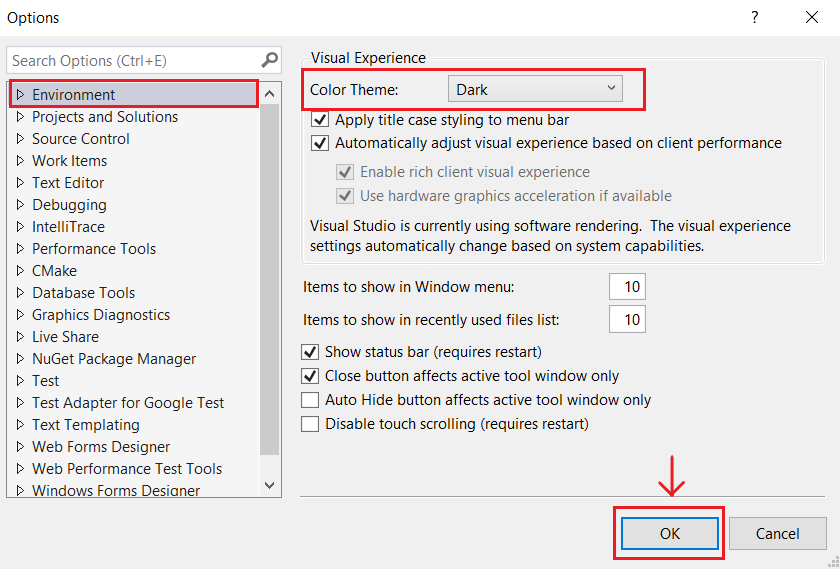
\includegraphics[scale=0.6]{img/dark}
\caption{Enabling the Dark Theme}\label{dark}
\end{figure}
\section{Hello World!}
We will now write our first C++ program.\\
Open Visual Studio. You will be prompted by a window. Select the option that says ``Create a new project" (See figure \ref{new_proj}).
\begin{figure}[h]
\centering
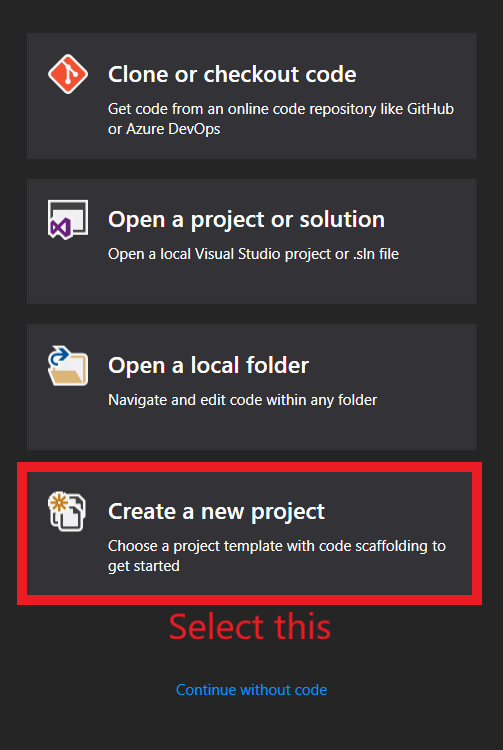
\includegraphics[scale=0.6]{img/new_proj}
\caption{Select ``Create a new project"}\label{new_proj}
\end{figure}
Now, select the option that says ``Windows Console Application". Click Next. Give your project a name and click on ``Create".
You should see something like this: (See figure \ref{vs})
\begin{figure}[h]
\centering
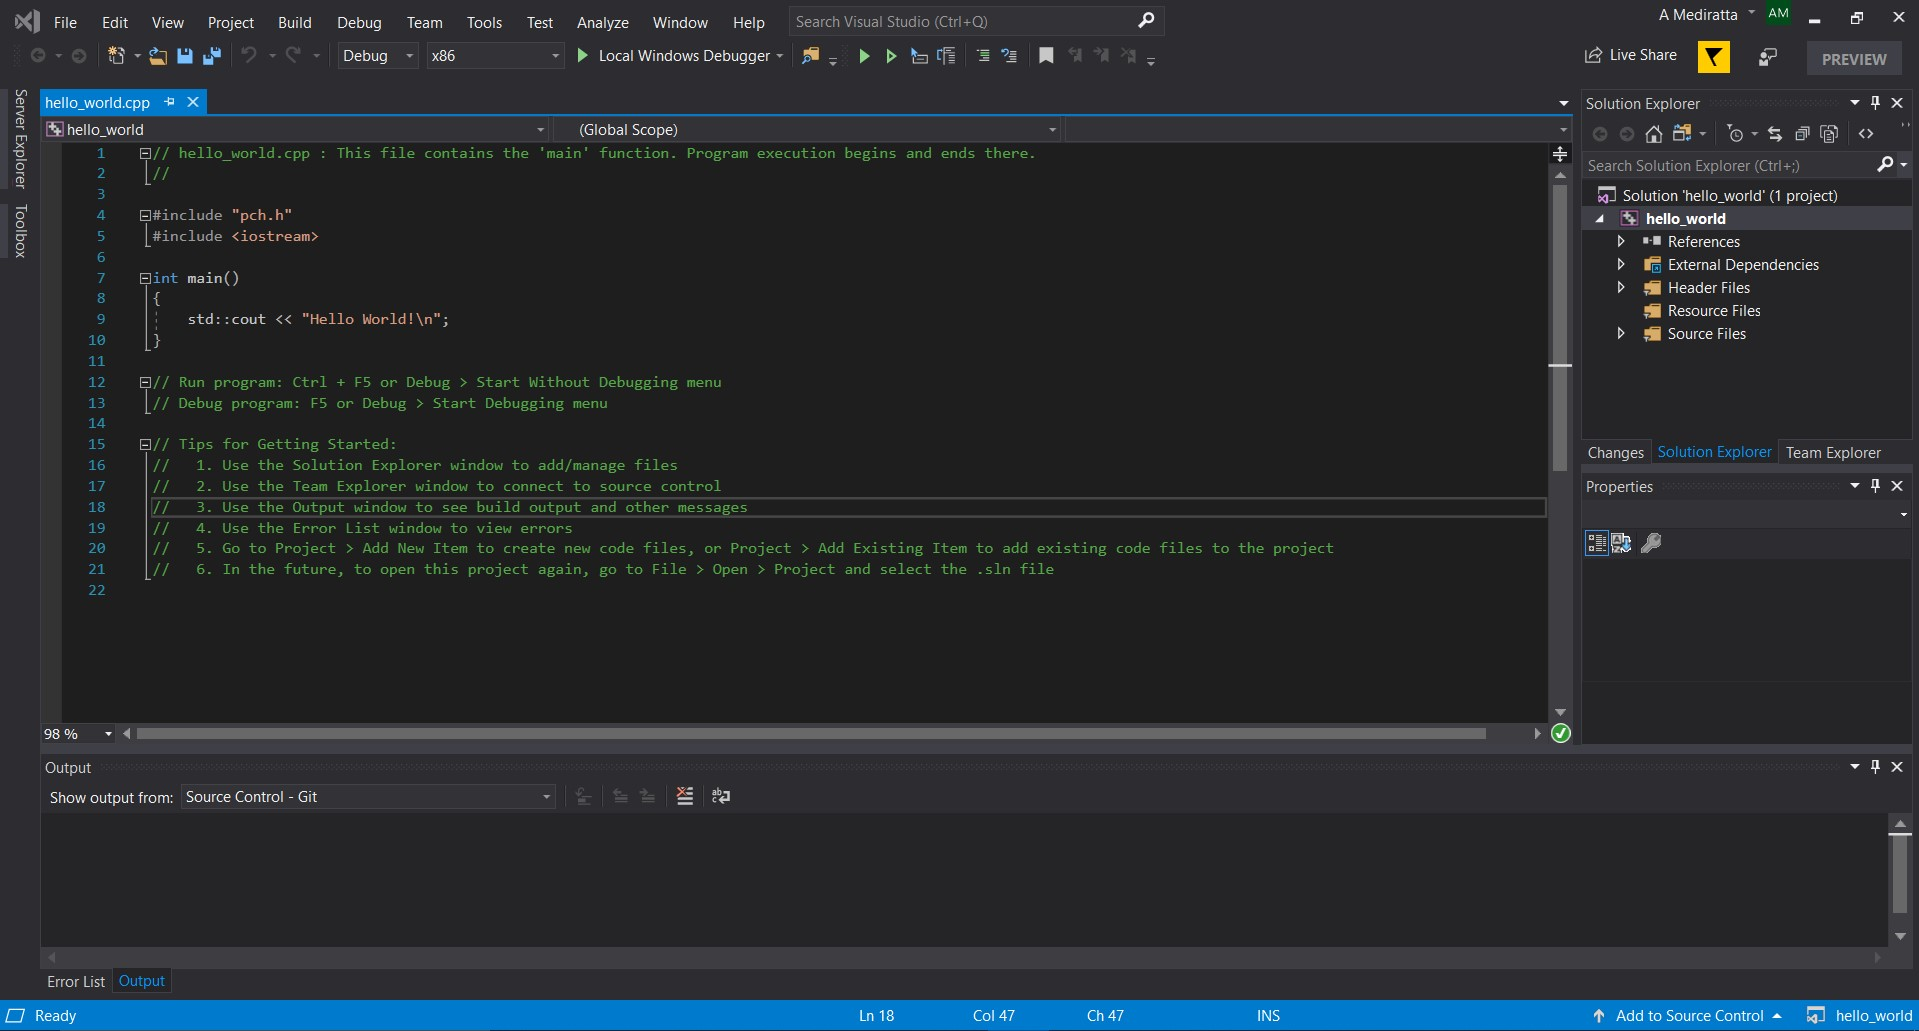
\includegraphics[scale=0.4]{img/vs}
\caption{New Project in Visual Studio}\label{vs}
\end{figure}
Now, delete everything other than the line that says \lstinline{#include "pch.h"} (or you might see \lstinline{#include "stdafx.h"}). We will talk about this later. It is not a part of the language itself - it is something specific to VS.\\
Now, enter the following code after that line:
\begin{lstlisting}
#include <iostream>
using namespace std;
int main()
{
	cout << "Hello World!" << endl;
}	
\end{lstlisting}
Now, press CTRL+F5. You will see a console window with the text ``Hello World!". Yeah! We made a computer display ``Hello World!" on screen. Let us now try to understand what each part of the code does.\\
Output:\\
\begin{lstlisting}
Hello World!
\end{lstlisting}
\section{Dissecting Hello World!}
\subsection*{The Preprocessor Include Directive}
Before I say anything about the preprocessor include directive, please understand that you do not need to worry about the name. It's just a fancy name for something really simple.\\
\lstinline{#include} is the preprocessor include directive.\\
A preprocessor directive is an instruction which are executed \textbf{before} your code is compiled.\\
In this case, we used the include directive to automatically copy and paste all the code that is there in a C++ library (header file) called \lstinline{iostream}.\\
All preprocessor directives start with a \lstinline{#} symbol (You can call it the sharp, the pound, the number symbol, the hash, the hashtag or even the octothorpe; I just call it the hash symbol).
\subsection*{The \lstinline{iostream} Library}
The \lstinline{iostream} header allows us to take input from and give output to the user. In our case, it provided us with the functionality to use \lstinline{cout} which allows us to display text on the screen and \lstinline{endl} which ends the line.
\subsection*{The Standard Namespace}
All C++ standard library features are enclosed in a container called the standard namespace or \lstinline{std}. The \lstinline{using namespace std;} part of the code allows us to tell the compiler that we are using the standard namespace. If we choose to not use that line in our code, we'd have to refer to all \lstinline{std} features with \lstinline{std::}, i.e. \lstinline{cout} would become \lstinline{std::cout} and \lstinline{endl} would become \lstinline{std::endl}.
\subsection*{The \lstinline{main()} function}
The main function (\lstinline{int main()}) defines what's called the entry point of the program. Code execution starts and ends with the main funcion.
\subsection*{The Curly Braces}
Curly braces \{\} in C++ define the start and end of something. In the Hello World program, you can see that we used the curly braces to define the start and the end of the main function. Anything that is enclosed within the curly braces is commonly called a ``block" of code.
\subsection*{The Semicolon}
Semicolons (;) in C++ denote the end of a complete statement. C++ gives us the ability to say a single statement in multiple lines and multiple statements in the same line. So when we are done with a complete statement, we use a semicolon to tell the compiler, ``Hey, I'm done describing this instruction. Whatever you see after this semicolon will be related to the next instruction."
You can roughly think about it as being analogous to the `full stop' (.) punctuation mark in English. (And French. And German. And other languages.)
\chapter{An Overview of Computer Science}
\epigraph{\centering ``Computer Science is no more about computers than astronomy is about telescopes."}{\textit{Edsger Dijkstra \\ Inventor of the Shortest Path Algorithm}}
This quote perfectly describes what most people think Computer Science is and shows where they go wrong. Computer Science is not about learning how to use computers. It is instead about computation - about understanding fundamentally how a computer processes information - and  about how we can make it better. It deals with the study of how efficient some algorithms are and how we can increase their efficiency.
\section{What is a computer anyway?}
Before I answer this question, I want you to think about where the word `computer' even comes from. Think about words that look or sound similar to the word `computer'.\\
Perhaps you thought of the verb `compute' and/or the noun `computation'.\\
But now, if you look up a dictionary, to compute means to calculate. From that analogy, a computer must be a calculator, right?
Here's what my teacher told me about a computer when I was in the third grade:
\begin{definition}
A \underline{computer} is an electronic device that takes input, processes it, and gives an output.
\end{definition}
While this definition is quite elegant and describes what a computer appears to do at the surface, we can go deeper.
\subsection{The Turing Machine}
\begin{figure}[h]
\centering
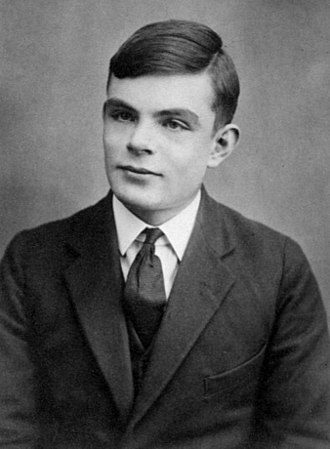
\includegraphics[scale=0.6]{img/turing}
\caption{Alan Turing}\label{turing}
\end{figure}
Say ``Hello" to Alan Turing! He was a great computer scientist... Oops! He was not just a computer scientist. Wikipedia describes him as an English mathematician, computer scientist, logician, cryptanalyst, philosopher and theoretical biologist (Whoa! That's way too many professions at once.).\\
So he is well known for his definition of a concept now known as the Turing Machine. A turing machine can be thought of as a hypothetical (imaginary) machine performing operations on data represented as a long series of zeroes and ones (which he described as a tape with blocks or cells that contained either a zero, or a one, or nothing).\\
Now, a turing machine can do the following things based on the instructions given to it:
\begin{itemize}
	\item Read what is stored at a particular cell. [Note that it can only be at one cell at a time.]
	\item Move left or right towards any given cell.
	\item Erase data from a cell.
	\item Write 0 or 1 at a given cell.
\end{itemize}
The initial state of the data is the \textbf{input} and what is left of the data after the Turing Machine has followed the instructions, is the \textbf{output}.
Now, while it might look most tasks a computer does can more-or-less be understood using the Turing Machine.\\
Scan this QR code to learn more about Turing Machines:\\
\begin{figure*}[h]
\centering
\qrcode[height=1.5in]{https://www.youtube.com/watch?v=dNRDvLACg5Q}
\caption{(https://www.youtube.com/watch?v=dNRDvLACg5Q)}
\end{figure*}
You will now see how the definition of the Turing Machine simply coincides with what we already know about. We will now revise some terms we have already learnt.
\subsection{Things we already know}
\begin{definition}
	The information a computer takes from the user for processing is called \underline{input}.
\end{definition}
\begin{definition}
	The information a computer gives back to the user after processing is called \underline{output}.
\end{definition}
The CPU has 2 main units:
\begin{itemize}
	\item ALU (Arithmetic and Logic Unit): it does all the math and makes the decisions.
	\item CU (Control Unit): it controls the input and output devices.
\end{itemize}
\section{Types of Knowledge}
In computer science, we divide knowledge into categories and primarily study a specific category of knowledge.\\
Knowledge exists in two types - Imperative and Declarative
\begin{definition}
Imperative knowledge is the type of knowledge that describes a procedure to do something - usually as a set of instructions.
\end{definition}
\begin{definition}
Declarative knowledge is the type of knowledge that states facts about something.
\end{definition}7
\section{Things to Keep in Mind}
\begin{itemize}
	\item Computers are deterministic machines.
	\item The output of a program is mostly predictable, unless it involves any randomization.
	\item They do exactly what they're told.
	\item If they don't do what you expected, it means you didn't tell them the right thing to do.
	\item In computer science, we study instructions given to the computer as algorithms, often represented as a flowchart or mostly using what's called pseudocode.
	\item Computers are dumb. However, they are very good at doing calculations and following your instructions quickly.
	\item A computer can do two types of calculations:
	\begin{itemize}
		\item The ones already defined in the language.
		\item The ones you define yourself.
	\end{itemize}
\end{itemize}
\chapter{Boolean Algebra}
\epigraph{\centering ``One should never try to prove anything that is not almost obvious."}{\textit{Alexander Grothendieck \\ French Mathematician, 1966 Fields Medallist}}
Boolean algebra is a concept of mathematics that helps us deal with statements about truth and allows us to formally talk about what is true and what is false.\\
Don't worry, I assure you that this is way easier than the mathematics you have studied until now. In fact, most of what we discuss here will seem to be common sense to you. And it is indeed common sense. It's just that we need a mathematical framework to talk about common sense.\\
In Computer Science, this concept is mostly referred to as ``Logic".\\
Yeah, we have a real defined meaning of the word ``Logic". Logic is simply a way of dealing with things that are either true or false.\\
\section{Some Background}
Boolean algebra is known to have been invented by George Boole (hence, the name ``Boolean").\\
But wait, did you notice how things in Boolean Algebra seem to be of two states (true and false), just like how binary is of two states (1 and 0)?\\
Even if you didn't, do these ideas look connected now?\\
Let me tell you that they are indeed well connected. Fun fact: One of the reasons why we made computers use the binary system is that Boolean Algebra existed much before computers did, and this helped us connect true to 1 and false to 0.\\
I hope you can now appreciate why we must study this strange branch of mathematics as a part of Computer Science.
\section{Variables}
A boolean variable can only have two values, a zero or a one. I will denote boolean variables as lower-case English letters, such as $a$, $b$, $c$, et cetera.
\section{A simple warm-up}
Before I explain how things work in Boolean Algebra, I want to show you how our intuition perfectly matches with what we're going to see.\\
As a warm-up exercise, state whether the following statements are true or false.\\
\begin{enumerate}
	\item $1 + 1 = 2$
	\item $90 \le 100$
	\item $1 + 5 > 9$ OR $2 + 2 = 4$
	\item $1 \times 0 = 100$
	\item In a right triangle, the square of the hypotenuse is NOT equal to the sum of the squares of the other two sides.
	\item Either you are wearing a red shirt OR you are NOT wearing a red shirt.
	\item If you toss a coin AND it lands on its circular face (not on its edge), then you will either get a Heads or a Tails.
\end{enumerate}
If you did this correctly like most people, you'll say that statements 1, 2, 3, 6 and 7 are true and the rest are false.
\section{Gates}
In Computer Science, a boolean operation is called a gate.\\
A gate can be looked at as something that takes one or two booleans as input and gives out a single boolean as an output.\\
If you study Boolean logic in Mathematics, you will find some complex notation. I will not use that notation here, so that you don't find yourself lost in the cumbersome notation and just get the idea of how things work. I hope that helps.
\subsection{The AND gate}
Don't worry, AND is not an abbreviation. It is literally the English Word ``and" written in ALL CAPS.\\
Boolean Algebra is best studied by making tables called \textbf{Truth Tables}.\\
Let us look at the truth table for the AND gate. Remember that 0 is false and 1 is true.
\begin{center}
	\begin{tabular}{ |c|c|c| } 
		\hline
		$a$ & $b$ & $a$ AND $b$ \\ 
		\hline
		0 & 0 & 0 \\ 
		0 & 1 & 0 \\
		1 & 0 & 0 \\
		1 & 1 & 1 \\
		\hline
	\end{tabular}
\end{center}
This describes the behaviour of the AND gate. The AND of two booleans is true if and only if both of them are true, i.e. $a$ AND $b$ = 1 $\Leftrightarrow a = 1, b = 1$.\\
If you think about it, this idea makes perfect sense. The whole statement ``I live in Delhi AND I know C++" is true if and only if both the individual statements ``I live in Delhi" and ``I know C++" are true. If any of these two statements is false, then the whole statement is false.
\subsection{The OR Gate}
Again, this is just the English word ``or", written in uppercase, not an abbreviation.\\
Let's look at the truth table of the OR gate.\\
\begin{center}
	\begin{tabular}{ |c|c|c| } 
		\hline
		$a$ & $b$ & $a$ OR $b$ \\ 
		\hline
		0 & 0 & 0 \\ 
		0 & 1 & 1 \\
		1 & 0 & 1 \\
		1 & 1 & 1 \\
		\hline
	\end{tabular}
\end{center}
From the table, we can see that the OR of two booleans is true if at least one of the two booleans is true. Even if both the booleans are true, the OR of the two booleans is true.\\
In more precise terms, this is the Inclusive OR Gate.
\subsection{The XOR Gate}
XOR stands for eXclusive OR.\\
Unlike the inclusive OR, the XOR gate returns false if both the statements are true.\\
\begin{center}
	\begin{tabular}{ |c|c|c| } 
		\hline
		$a$ & $b$ & $a$ XOR $b$ \\ 
		\hline
		0 & 0 & 0 \\ 
		0 & 1 & 1 \\
		1 & 0 & 1 \\
		1 & 1 & 0 \\
		\hline
	\end{tabular}
\end{center}
It returns true if out of the two statements, strictly one of them is true. If both are true, the overall XOR statement is false.
\subsection{The NOT gate}
Unlike the other gates, the NOT gate takes only one boolean as input and returns the negative of that input, i.e. NOT true = false and NOT false = true.
\begin{center}
	\begin{tabular}{ |c|c| } 
		\hline
		$a$ & NOT $a$ \\ 
		\hline 
		0 & 1 \\
		1 & 0 \\
		\hline
	\end{tabular}
\end{center}
\section{Boolean Identities}
The proofs of these identities are trivial. You can prove these by making a truth table for the LHS and the RHS. You do not need to remember any of this, but make sure you understand what they mean, or at least verify if they look obvious (spoiler alert: they will).\\
\begin{align}
a \text{ OR } b &= b \text{ OR } a\\
a \text{ AND } b &= b \text{ AND } a\\
a \text{ XOR } b &= b \text{ XOR } a\\
a \text{ OR } (b \text{ OR } c) &= (a \text{ OR } b) \text{ OR } c\\
a \text{ AND } (b \text{ AND } c) &= (a \text{ AND } b) \text{ AND } c\\
a \text{ AND } (b \text{ OR } c) &= (a \text{ AND } b) \text{ OR } (a \text{ AND } c)\\
a \text{ OR } 0 &= a\\
a \text{ OR } 1 &= 1\\
a \text{ AND } 0 &= 0\\
a \text{ AND } 1 &= a\\
a \text{ AND } (a \text{ OR } b) &= a\\
a \text{ OR } (a \text{ AND } b) &= a\\
(\text{ NOT } a) \text{ AND } (\text{ NOT } B) &= \text{ NOT }(A \text{ OR } B)\\
(\text{ NOT } a) \text{ OR } (\text{ NOT } B) &= \text{ NOT }(A \text{ AND } B)\\
a \text{ AND } (\text{ NOT } a) &= 0\\
a \text{ OR } (\text{ NOT } a) &= 1
\end{align}
\section{Boolean Algebra and Set Theory}
You will realise in class 11 mathematics that most of what we just learnt is basically applied in another completely different field in mathematics called Set Theory.\\
The idea of OR translates to the union of two sets. The idea of AND translates to the intersection of two sets and the idea of NOT translates to the complement of a set.\\
The identities we just learnt will have a direct application in both programming and set theory. In fact, most of these identities (other than the ones involving 0 and 1) are basically the same as those they teach in Set Theory.\\
Each of these identities has a name, but I don't want to confuse you with that :).
\chapter{C++ From Scratch}
\epigraph{\centering ``A computer will do what you tell it to do, but that may be different from what you had in mind."}{\textit{Joseph Weizenbaum \\ One of the fathers of modern artificial intelligence}}
\section{The language}
C++ is a compiled language. This means that there exists a piece of software called the compiler that takes your source code and ``compiles" it into machine-readable code in an executable format supported by the operating system. For Windows, this is the .exe executable format. For *nix based systems, this is mostly the .out format.\\
The standard libraries are huge repositories of code written in perfectly normal C++ and provide us with various functionalities. However, there are other entities in C++ which are built into the language itself.\\
\section{The Minimal Program}
The minimal C++ program looks like this:\\
\begin{lstlisting}
int main() {}
\end{lstlisting}
This is the essential bare-minimum for a program to be valid C++. What does this code do? Nothing. It literally just declares a \textbf{function} called ``main" and does not define anything inside the function.\\
The curly braces \{\} denote the start and end of a code block. In this case, the code block is used to enclose the contents of the \lstinline{main()} function. 
\section{Console Output}
In our first C++ program, we made the computer display ``Hello World!" on the screen. For a recap, this was the program:
\begin{lstlisting}
#include <iostream>
int main()
{
	std::cout << "Hello World!" << std::endl;
	return 0;
}
\end{lstlisting}
In the beginning, we included a header file called \lstinline{iostream} which enables us to display output to and take input from the user.\\
Now, here's what I want you to try. You know that we made the computer display ``Hello World!". It must be visible to you that we could otherwise make it display anything we like. So, go ahead and try to replace that text inside the quotes with something else of your choice and see what happens when you compile and run it. If you successfully changed the text, it would have displayed the new text you changed.\\
Great job! You can now make the computer display whatever you like.\\
\begin{remark}
In fact, the name \lstinline{iostream} literally speaks for itself. I/O is the abbreviated form of Input/Output.
\end{remark}
Here's another experiment I want you to try.\\
Remove the quotes surrounding the text and now try to compile the program.\\
You will now see an error. (depending on which distribution of C++ you use). That's sad :(\\
But now, try replace that text with 2+2, i.e.\\
\begin{lstlisting}
#include <iostream>
int main()
{
	std::cout << 2+2 << std::endl;
	return 0;
}
\end{lstlisting}
You'll see that this program works, even without the quotes and in fact, this time, it displayed 4.\\
\lstinline{std::cout} is a \textbf{keyword} in the \lstinline{iostream} library that is used to display output to the console and \lstinline{std::endl} is used to end the line.
\section{Comments}
We often have to mark certain parts of our code so that we remember what that does or so that other people can understand our code easily. This is done through comments.\\
Any part of the code that is commented is not read by the C++ compiler and is ignored. It only helps humans understand the code better.\\
There are two types of comments allowed in C++: Single-line comments and Multi-line comments.
\subsection{Single-line comments}
Single-line comments, as the name suggests, span upto the current line. Single-line comments made with two forward slashes (//).\\
For example:
\begin{lstlisting}
// This is a single-line comment
// This is another single-line comment
\end{lstlisting}
Note that single-line comments can start from any point in the line, and extend for that whole line.\\
Therefore, if a single line comment can start right after a piece of code and that code will still be executed.\\
Example:
\begin{lstlisting}
std::cout << "ABC" << std::endl; // comment 
\end{lstlisting}
\subsection{Multi-line comments}
Multi-line comments start with a \textbf{/*} and end with a \textbf{*/}.\\
Example:
\begin{lstlisting}
/* This is
a multi-line
comment */
\end{lstlisting}
\section{Variables}
When you read this word ``Variables", it might remind you of algebra. However, the notion of a variable is similar, yet quite different in computer science compared to what you've learnt in algebra.\\
\subsection{A Useful Analogy}
With time, you will realise for yourself what a variable actually is. However, since you are probably new to programming in general, here's a useful analogy that works. Whenever you're stuck, this analogy will help you.\\
Whenever I say, ``Variable", imagine a \textbf{bucket} that can store a particular type of information. We can read the information stored in a variable (bucket) and change it.\\
This idea is very important - We can change the data stored in a variable by assigning it a new value.
\subsection{Declaring Variables}
Now that you know what I mean by variables, we can now start playing with variables.\\
Here's how we declare a variable in C++.\\
We first mention the keyword corresponding to the datatype, i.e. the type of information we want to store in the bucket and then the name of the variable. These are some of the datatypes C++ supported by default:
\begin{center}
	\begin{tabular}{ |c|l| } 
		\hline
		Keyword & Datatype \\ 
		\hline
		bool & Boolean (true or false)\\
		int & Integer (Ex. 2, 1000, -282)\\
		char & Character (Ex. `a', `@', `N')\\
		float & Floating-point decimal (Ex. 2.292)\\
		double & Double-precision floating point decimal (Ex. 39.329034)\\
		\hline
	\end{tabular}
\end{center}
Example variable declaration:
\begin{lstlisting}
int myNumber;
\end{lstlisting}
The assignment operator (=) is used to assign a value to a variable.\\
Example:
\begin{lstlisting}
bool isHappy; // Creates a boolean variable
isHappy = true; // Assigns value true to isHappy
\end{lstlisting}
The two lines of code above can combined into a single statement.
\begin{lstlisting}
bool isHappy = true;
\end{lstlisting}
Like in the above line, when we create a variable and assign it a value within its declaration, it's called initialization. It's considered a good practice to always initialize your variables with a value. Another way to initialize a variable is the following:
\begin{lstlisting}
int myNumber {1};
\end{lstlisting}
Note that although you can initialize a variable like this, you cannot assign a value to variable using curly braces. For assignment, the equal sign must be used.\\
Also, by the modern C++ Core Guidelines, it is considered as a good practice to use curly braces for initialization (i.e. the last method).
\section{Operators and Operands}
You know what an operator is in mathematics. We have four main arithmetic operators in math for addition($+$), subtraction($-$), multiplication($\times$) and division($\div$). Similarly, we have operators in C++.
\begin{definition}
	An \underline{operator} is a symbol that tells the computer to perform some specific \underline{operation}. 
\end{definition}
\begin{definition}
	\underline{Operands} are the values that the operation performed by an operator takes.
\end{definition}
Unlike most other languages, C++ allows us to have custom operators. However, we won't discuss custom operators here.\\
C++ has many operators built-in.\\
Let's look at some of them.
\subsection{The assignment operator}
The equal sign ($=$) is the assignment operator in C++, as discussed before. It assigns values to variables. However, it must not be taken like the equality symbol in mathematics. What you are going to see now is a valid C++ program.
\begin{lstlisting}
#include <iostream>
int main()
{
	int a {1};
	a = 6; // Yes, this is valid.
	std::cout << a << std::endl;
	return 0;
}
\end{lstlisting}
What do you think will be the output of this program? The variable $a$ had been assigned a value before being assigned a value of 6. Now if you see it like mathematics, it doesn't make sense. We can't say $a = 1$ and $a = 6$ at the same time.\\
This is where the bucket analogy will help. Consider a bucket that had the number 1 in it. Then, it was emptied and 6 was put in it.\\
\textbf{Therefore, the output of this program will be 6.}
\subsection{The arithmetic operators}
\subsubsection{The addition operator}
As the name suggests, the addition operator can add two variables or literal numbers.\\
The symbol for addition is the `plus' sign ($+$).
\begin{remark}
	The plus sign ($+$) does not only do the work of addition. It has multiple uses, as we will see later.
\end{remark}
Look at this example:
\begin{lstlisting}
#include <iostream>
int main()
{
	int a {6};
	int b {5};
	std::cout << a + b << std::endl; // This will output 11
	return 0;
}
\end{lstlisting}
If you compile and run this, you'll get the output as 11. The reason should be obvious. We know that when we add 6 and 5, we will get 11.\\
Now, think about this. What will this piece of code do?
\begin{lstlisting}
#include <iostream>
int main()
{
	int a {6};
	a = a + 2;
	std::cout << a << std::endl;
	return 0;
}
\end{lstlisting}
We made a new variable (bucket) and gave it the value 6. Then, we said \lstinline{a = a + 2;}. If this confuses you, don't worry. Just remember that this is not an algebraic equation. It is an \textbf{instruction} to the computer. What it does is that it sets the value of the variable \lstinline{a} to a new value which is exactly two more than its initial value.\\
Therefore, the output of the above program will be $8$, since $6 + 2 = 8$.\\
We will soon find that there is another operator to do exactly that, and requires us to type less. However, if I had just shown you what that operator did, you'd never know anything like \lstinline{a = a + 2;} is possible. That's the fun of learning. First, you learn it the hard way; and then, once you've understood how things work, you learn it the easy way.
\subsubsection{The Subtraction operator}
Again, you probably know what it does, but let me still say it.\\
The subtraction operator finds the difference between the first and second values it is provided with.\\
The hyphen symbol (or the minus sign), ($-$) is the subtraction operator.\\
Look at this example:
\begin{lstlisting}
#include <iostream>
int main()
{
	int a {6};
	int b {5};
	std::cout << a - b << std::endl; // This will output 1
	return 0;
}
\end{lstlisting}
Again, we know that $6 - 5 = 1$, therefore, the output of this program will be 1. Note that if $a$ were smaller than $b$, you would've got a negative number (obviously).
\subsubsection{The Multiplication operator}
The multiplication operator multiplies the two types of numbers it receives.\\
The asterisk symbol ($*$) is the multiplication operator in C++.\\
This example will explain that:
\begin{lstlisting}
#include <iostream>
int main()
{
	int a {6};
	int b {5};
	std::cout << a * b << std::endl; // This will output 30
	return 0;
}
\end{lstlisting}
Clearly, $6 \times 5 = 30$, therefore, the program will output 30.
\subsubsection{The Division operator}
The division operator divides the two types of numbers it receives.\\
The forward slash symbol ($/$) is the division operator in C++.\\
However, there's a small catch. When the division operator is applied on two integers, it returns an integer. This means, you will only get the \textbf{quotient} of division.\\
Though it will return a decimal answer if it is supplied with two \lstinline{double}s or \lstinline{float}s.
This example will explain that:
\begin{lstlisting}
#include <iostream>
int main()
{
	int a {6};
	int b {5};
	std::cout << a / b << std::endl; // This will output 30
	return 0;
}
\end{lstlisting}
Clearly, $\frac{6}{5}$ gives quotient $1$, therefore, the program will output 1.\\
But now look at this:
\begin{lstlisting}
#include <iostream>
int main()
{
	double a = 5.0;
	double b = 2.0;
	std::cout << a / b << std::endl; // This will output 2.5
	return 0;
}
\end{lstlisting}
The output of this program will be $2.5$. This is because we are dividing two floating point decimal numbers.
\subsubsection{The Modulo Operator}
The modulo operator finds the \textbf{remainder} when the two numbers received by it are divided.\\
The symbol for this operator is the per cent sign (\%). Note that this operator is only defined for integers.
\begin{lstlisting}
#include <iostream>
int main()
{
	int a {8};
	int b {3};
	std::cout << a % b << std::endl; // This will output 2
	return 0;
}
\end{lstlisting}
The output of this program will be two because when you divide 8 by 3, the remainder you get is 2, because $8 = (3 \times 2) + 2$.
\subsection{Boolean Operators}
Remember we studied boolean algebra (see Chapter 2)? The logic ``gates" we studied there are built-in operations in C++.
\subsubsection{The OR operator}
The OR operator takes the OR of two boolean values.\\
The symbol for it is two vertical pipe symbols ($||$).\\
Look at this program:
\begin{lstlisting}
#include <iostream>
int main()
{
	bool a {true};
	bool b {false};
	std::cout << a || b << std::endl;
	return 0;
}
\end{lstlisting}
You will see that this program outputs 1, which is the same as the boolean `true'.
\subsubsection{Other Boolean Operators}
By now, you would've got an idea of how operators work. So let me just show you a quick table of all C++ boolean operators, so that you can try to use them.
\begin{center}
	\begin{tabular}{ |c|c| } 
		\hline
		Operation & Operator\\
		\hline
		AND & \& \& \\ 
		NOT & $!$ \\
		\hline
	\end{tabular}
\end{center}
And well, that's it! The XOR gate is just a combination of AND, OR and NOT.\\
Basically, $a \text{ XOR } b = [a \text{ AND } (\text{ NOT } b )] \text{ OR } [b \text{ AND } (\text{ NOT } a )]$\\
\subsection{Comparison Operators}
Here's a table of the comparison operators in C++. You'll find them quite simple. They return a boolean value (\lstinline{true} or \lstinline{false}), based on whether the whole statement is \lstinline{true} or \lstinline{false}.
\begin{center}
	\begin{tabular}{ |c|c| } 
		\hline
		Operator on x and y & Comparison\\
		\hline
		x == y & equal\\
		x != y & not equal to\\
		x $<$ y  & less than\\
		x $>$ y  & greater than\\
		x $<=$ y & less than or equal to\\
		x $>=$ y & greater than or equal to\\
		\hline
	\end{tabular}
\end{center}
\subsection{End Note on Operators}
These are not the only operators in C++. We will talk about more operators later. In fact, C++ is so flexible that it even allows custom operators.\\
Also, you can always use multiple operators in the same instruction. When you do that, you can use parentheses, i.e. round brackets () to specify which operation is to be done first. For example:
\begin{lstlisting}
#include <iostream>
int main()
{
	std::cout << ((2 + 2) - 1) << std::endl;
	return 0;
}
\end{lstlisting}
This program will output 3 since $2 + 2$ is $4$. Subtract one, and that's $3$. (Quick Math!)\\
So the output will be 3.
\end{document}